\chapter{Introdução}
\label{chap:intro}

Este capítulo apresenta a organização do trabalho e contextualiza a justificativa e a relevância sobre o tema desta dissertação. 

 \section{Organização do trabalho}
\label{organizacao}

O presente trabalho é organizado nos seguintes capítulos:

\begin{itemize}
    \item Capítulo \ref{chap:intro}: Introdução - que apresenta a motivação, a contextualização, os objetivos e a organização do trabalho;
    \item Capítulo \ref{chap:historicoversoes}: Sistema de Ingresso e Versionamento - que elenca o histórico de mudanças no sistema de cotas do sistema de ingresso do \gls{IFSC}, o que motivou o estudo inicial desta pesquisa;
    
    \item Capítulo \ref{chap:fundamentacao}: Fundamentação Teórica - o qual aborda a revisão da literatura sobre os temas ligados ao desenvolvimento de \gls{DSL} na engenharia de software, as diferenças sobre \gls{GPL}, as vantagens e desvantagens do uso  \gls{DSL}, assim como as ferramentas utilizadas para a sua construção;
        
    \item Capítulo \ref{metodologia}: Metodologia - no qual é descrita a classificação e as etapas da pesquisa, o ambiente da pesquisa e os métodos de avaliação da DSL;

    \item Capítulo \ref{chap:dslcotas}: DSL de Cotas - que aborda uma \gls{DSL} como meio de simplificar a especificação e desenvolvimento de regras de classificação de candidatos ao sistema de cotas da rede de ensino pública federal, assim como apresenta a \gls{API} DSL Cotas, responsável por implementar o serviço de classificação e aprovação de candidatos;
    \item Capítulo \ref{chap:analise}: Avaliação e Análise dos Resultados - o qual contém a análise dos dados coletados por meio de um exercício prático de avaliação da DSL Cotas, de um questionário aplicado com os usuários e da avaliação da
    \gls{API} DSL Cotas;
    \item Capítulo \ref{chap:consideracoes}: Conclusões - na qual é realizada uma síntese dos principais resultados da pesquisa, bem como os trabalhos relacionados, o espoco negativo da pesquisa, as principais contribuições da DSL Cotas, os trabalhos futuros sugeridos e as considerações finais.
\end{itemize}


Nas seções \ref{contextualizacao} e \ref{motivacao} serão abordados os elementos contextuais e motivacionais para desenvolvimento desse estudo, enquanto nas seções \ref{problema} e \ref{objetivos} serão apontados o problema, as hipóteses e os objetivos da pesquisa. Por fim, na seção \ref{metodologia} serão definidos os métodos utilizados.


 \section{Contextualização}
\label{contextualizacao}

 Para \citeonline{ghosh2011dsl}, problemas na comunicação entre desenvolvedores e especialistas de domínio são os principais motivos de falha no desenvolvimento e evolução de projetos de software. Especialistas, entendem a terminologia do domínio e falam em um vocabulário que pode ser estranho para as equipes de desenvolvedores. Nesse sentido, é preciso identificar meios para redução da lacuna semântica entre especialistas e desenvolvedores, de modo que os especialistas possam estar envolvidos na verificação de regras de negócio ao longo do ciclo de vida do projeto.

 A constante alteração de regras de negócio advém de mudanças de lei, forças de mercado ou novos objetivos empresariais, exigindo que essas possam ser expressas de modo a serem compreendidas e facilmente alteradas pelas organizações, a fim de melhorar o desempenho de negócios \cite{flexiblerules}.
 
 Segundo \citeonline{verificationbusinessrules}, a mudança de regras de negócio é inevitável, sendo cada vez mais frequente a adaptação às novas regulamentações e a necessidade de os sistemas estarem em conformidade com novas regras, que por décadas são implementadas em softwares de áreas industriais, financeiras, empresas de seguros, administração e várias outras.
 
 O \gls{IFSC} é uma instituição da rede de ensino pública federal presente no estado de Santa Catarina há mais de 100 anos, que hoje desenvolve e mantém diversos sistemas de informação, os quais estão sujeitos a alterações para conformidade à legislação federal. As aplicações institucionais têm como principais envolvidos os discentes, os professores e os técnicos administrativos, que participam da oferta de cursos nos mais diversos níveis, tais como cursos de qualificação profissional, educação jovens e adultos, técnicos, superiores e pós-graduação. 
 
 Ao que concerne à necessidade de adaptação a novas regras de negócio, o autor da presente pesquisa trata sobre um dos sistemas de informação mais utilizados internamente, o sistema de ingresso de discentes na instituição, o qual é mantido desde 2007 pela \gls{DTIC} e tem como objetivo disponibilizar ofertas de vagas em cursos por meio de processos seletivos. Atualmente, a base de dados do sistema conta com 788 processos seletivos e mais de 409 mil registros de candidatos.
 
 A principal funcionalidade do sistema de ingresso do \gls{IFSC} é a classificação de candidatos, a qual é construída e mantida conforme critérios da Lei nº 12.711/2012, que estabelece:
 \begin{citacao}
 Art. 1º As instituições federais de educação superior vinculadas ao Ministério da Educação reservarão, em cada concurso seletivo para ingresso nos cursos de graduação, por curso e turno, no mínimo 50\% (cinquenta por cento) de suas vagas para estudantes que tenham cursado integralmente o ensino médio em escolas públicas.
 
 Art. 3º Em cada instituição federal de ensino superior, as vagas de que trata o art. 1º desta Lei serão preenchidas, por curso e turno, por autodeclarados pretos, pardos e indígenas e por pessoas com deficiência, nos termos da legislação, em proporção ao total de vagas no mínimo igual à proporção respectiva de pretos, pardos, indígenas e pessoas com deficiência na população da unidade da Federação onde está instalada a instituição, segundo o último censo da Fundação Instituto Brasileiro de Geografia e Estatística - IBGE \cite{leicotas}.  
 \end{citacao}
 
 A adequação à legislação é demanda proveniente do \gls{MEC}, o qual faz referência em seu site aos decretos nº 7.824/2012, nº 9.034/2017 (que regulamentam a lei nº12.711) e às portarias normativas nº 18/2012 e nº 9/2017, as quais estabelecem regras, conceitos básicos e fórmulas para preenchimento das modalidades de reservas de vagas do sistema de cotas. 
 
 Sempre que o \gls{MEC} realiza alterações em um dos documentos de lei citados, é necessário também alterar os sistemas de informações das instituições de ensino. A exigência para adequação dos sistemas à lei traz o aumento da demanda de desenvolvimento, situação ilustrada no Capítulo  \ref{chap:historicoversoes}, no qual é elencado o histórico do controle de versão para 3 (três) versões já implementadas no \gls{IFSC}.
 
 

 
 

 \section{Motivação}
\label{motivacao}

O estudo de linguagens que sejam capazes de expressar regras de maneira mais clara não é novidade na área da engenharia de sistemas. \citeonline{bentley} já demonstrava em sua pesquisa diferentes abordagens de construção de pequenas linguagens para facilitar a escrita de programas gráficos e interface gráfica.


\citeonline{wexelblat}, apresenta o termo "linguagem de propósito especial", quando se refere à \gls{JOVIAL}, linguagem de alto nível destinada principalmente para auxiliar na programação de grandes sistemas complexos em tempo real. 

Um exemplo de aplicação dessas linguagens pode ser visto na Figura \ref{fig:piclanguage} em que o compilador transforma comandos simples no formato textual em formato de digrama (Figura \ref{fig:piclanguageresultado}), abstraindo detalhes específicos das linguagens tradicionais de programação da época.

\begin{figure}[ht!]
\centering

\caption{\textmd{Comandos na PIC Language}}
\label{fig:piclanguage}
\fcolorbox{gray}{white}{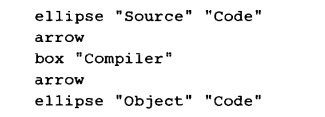
\includegraphics[width=0.67\textwidth]{images/piclanguage}}

\par\medskip\textbf{Fonte:} \citeonline{bentley}. \par\medskip
\end{figure}

\begin{figure}[ht!]
\centering

\caption{\textmd{Diagrama resultado após compilação}}
\label{fig:piclanguageresultado}
\fcolorbox{gray}{white}{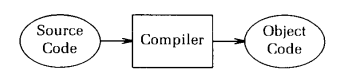
\includegraphics[width=0.67\textwidth]{images/piclanguageresultado}}

\par\medskip\textbf{Fonte:} \citeonline{bentley}. \par\medskip
\end{figure}



Na engenharia de software atual, as Linguagens de Domínio Específico ou DSLs, do inglês \textit{Domain Specific Languages}, estão se tornando cada vez mais importantes e as novas ferramentas de criação dessas linguagens tem evoluído, reduzindo o esforço de desenvolvimento \cite{dslengineering}.


A equipe de desenvolvedores do \gls{IFSC} possui uma alta demanda de desenvolvimento de sistemas e serviços internos, atualmente são mantidos mais de 10 sistemas em uso, alguns deles subdivididos em vários módulos \cite{catalogoifsc}. A \gls{DTIC} centraliza e mantém a maioria dos sistemas e serviços de TI, contando com apenas 12 analistas da tecnologia da informação, além de prestar suporte para todas as 23 unidades da instituição. 

Como agravante, o sistema de ingresso foco deste trabalho, foi criado em meados dos anos 2000 por bolsistas que já não estão mais na instituição, e atualmente apenas 2 (dois) desenvolvedores são responsáveis pelas demandas de desenvolvimento e suporte. Por se tratar de um sistema legado criado em linguagem PHP sem qualquer preocupação com documentação ou qualidade de código, o custo de alterações mais complexas como no caso de regras de classificação acaba por atrasar a adequação aos novos requisitos de lei. 

Até o momento, a presente equipe participou do desenvolvimento de 3 (três) versões do algoritmo de classificação, além de prestar manutenção corretiva em função de entendimentos equivocados nas regras implementadas.  Os algoritmos envolvidos, assim como o seu histórico de versionamento são detalhados no Capítulo \ref{chap:historicoversoes}.

Essa pesquisa apresenta uma Linguagem de Domínio Específico que permite a especificação de regras de classificação de candidatos, na qual usuários especialistas do sistema de ingresso possam estabelecer as categorias de cotas, com objetivo de reduzir o esforço do desenvolvimento e de entendimento das regras de negócio por parte de usuários e de desenvolvedores. 

Nas Seções \ref{problema}, \ref{objetivos} e \ref{organizacao}, são apresentados, respectivamente, o problema de pesquisa e as hipóteses, os objetivos e, por fim, a organização do trabalho.

  
  \section{Problema de pesquisa e Hipótese}
\label{problema}

Essa pesquisa surge em decorrência das necessidades recentes para refatoração do código fonte do sistema de ingresso do \gls{IFSC}. Essas necessidades, foram resultadas em função de alterações nos documentos de lei e em função de  divergências sobre o entendimento de distribuição de vagas entre desenvolvedores e especialistas de negócio. O que acaba por muitas vezes atrasando o processo de implementação do sistema para aderência a uma nova legislação ou a uma instrução normativa definida pelos órgãos de controle.

Essas situações, trazem alguns desafios para a equipe de desenvolvedores e para os \textit{stakeholders} que analisam a legislação e definem os requisitos do sistema de convocação de candidatos cotistas nos cursos do \gls{IFSC}. 

No que concerne o apoio ao desenvolvimento e especificação desse problema de pesquisa, podem ser listados os seguintes questionamentos:

\begin{itemize}
    \item Como dar liberdade aos usuários para definir as regras do sistema de cotas, e utilizar essas definições de modo a serem implantadas diminuindo a dependência da equipe de  desenvolvedores?
    
    \item É possível que a criação de uma linguagem específica de domínio que padronize as definições em comum nas regras de distribuição de vagas?
    
    \item A utilização da linguagem proposta pode reduzir a quantidade de linhas de código a serem implementadas manualmente pelos desenvolvedores?
    
    \item Quais são as ferramentas utilizadas para construção de \gls{DSL}s e de que modo podem permitir a geração de código fonte para implementação do algoritmo de classificação por cotas?
    
    \item A definição de regras do sistema de cotas pode ser facilitada com apoio de uma \gls{IDE} que faça validações e forneça recursos específicos para a linguagem proposta?
    

    
\end{itemize}{}
 
 \section{Objetivos}
\label{objetivos}

\subsection{Objetivo Geral}
\label{objetivogeral}

Compreender, por meio da elaboração de uma linguagem específica de domínio, a viabilidade de melhoria na comunicação entre usuários de negócio e desenvolvedores, visando o aumento na produtividade da especificação de requisitos e da implementação de regras concernentes ao sistema de cotas da rede de ensino pública federal. 


\subsection{Objetivos Específicos}
\label{objetivosespecificos}

\begin{enumerate}
    \item[a)] Realizar levantamento do histórico de versões presentes no sistema de controle de versão do \gls{IFSC} sobre regras de classificação de cotas;
    \item[b)] Analisar e identificar características em comum entre as versões do algoritmo implementadas para que seja possível elaborar a modelagem da \gls{DSL} proposta;
    \item[c)] Definir e implementar uma \gls{DSL} para usuários especialistas nas regras do sistema de cotas;
    \item[d)] Criar um cenário de avaliação da DSL, a fim de validar a sua usabilidade os usuários de negócio;
    \item[e)] Implementar uma \gls{API} utilizando as regras definidas pelos usuários de negócio, para geração do algoritmo de classificação pelo sistema de cotas.
\end{enumerate}{}
      
 \section{Metodologia}
\label{metodologia}

A elaboração dessa pesquisa, utilizará como metodologias:

\begin{enumerate}
    \item[a)] Revisão bibliográfica - sobre o levantamento do estado da arte de conceitos relacionados a modelagem de \gls{DSL}s;
    
    \item[b)] Pesquisa documental - no que concerne à análise do histórico do controle de versão do \gls{IFSC} relacionando as alterações realizadas em função de documentos de lei ou em função de demandas dos envolvidos no processo de classificação de candidatos.
    
\end{enumerate}

Por fim, para avaliação desse estudo será realizado um experimento com os principais \textit{stakeholders} do IFSC envolvidos na definição de requisitos da lei. Essa avaliação visa identificar a usabilidade da \gls{DSL} proposta.

 
% \section{Organização do trabalho}
\label{organizacao}

O presente trabalho é organizado nos seguintes capítulos:

\begin{itemize}
    \item Capítulo \ref{chap:intro}: Introdução - que apresenta a motivação, a contextualização, os objetivos e a organização do trabalho;
    \item Capítulo \ref{chap:historicoversoes}: Sistema de Ingresso e Versionamento - que elenca o histórico de mudanças no sistema de cotas do sistema de ingresso do \gls{IFSC}, o que motivou o estudo inicial desta pesquisa;
    
    \item Capítulo \ref{chap:fundamentacao}: Fundamentação Teórica - o qual aborda a revisão da literatura sobre os temas ligados ao desenvolvimento de \gls{DSL} na engenharia de software, as diferenças sobre \gls{GPL}, as vantagens e desvantagens do uso  \gls{DSL}, assim como as ferramentas utilizadas para a sua construção;
        
    \item Capítulo \ref{metodologia}: Metodologia - no qual é descrita a classificação e as etapas da pesquisa, o ambiente da pesquisa e os métodos de avaliação da DSL;

    \item Capítulo \ref{chap:dslcotas}: DSL de Cotas - que aborda uma \gls{DSL} como meio de simplificar a especificação e desenvolvimento de regras de classificação de candidatos ao sistema de cotas da rede de ensino pública federal, assim como apresenta a \gls{API} DSL Cotas, responsável por implementar o serviço de classificação e aprovação de candidatos;
    \item Capítulo \ref{chap:analise}: Avaliação e Análise dos Resultados - o qual contém a análise dos dados coletados por meio de um exercício prático de avaliação da DSL Cotas, de um questionário aplicado com os usuários e da avaliação da
    \gls{API} DSL Cotas;
    \item Capítulo \ref{chap:consideracoes}: Conclusões - na qual é realizada uma síntese dos principais resultados da pesquisa, bem como os trabalhos relacionados, o espoco negativo da pesquisa, as principais contribuições da DSL Cotas, os trabalhos futuros sugeridos e as considerações finais.
\end{itemize}

 
% \input{figures/densenet}

%\input{equations/ce}

%\input{tables/deep_datasets}

% \input{algorithms/algorithm} 
